\question{Câu 2}

Thiết kế mạch tổ hợp tìm vị trí bit 1 đầu tiên (tính từ MSB) của chuỗi 24-bit. Cho các standard cell như sau: cổng not, các cổng logic 2 ngõ vào, mux 2-1, mux 4-1.

\answer{a}{Thiết kế mạch chỉ được dùng các standard cell trên.}

Đầu tiên nhóm em sẽ thiết kế từ một bộ tìm kiếm vị trí bit 1 đầu tiên (tính từ MSB) cho một chuỗi 4-bit trước. 

\begin{table}[H]
	\centering
	\begin{tabular}{|c|c|c|c|c|c|c|}
		\hline
		\multicolumn{4}{|c|}{Input} & \multicolumn{2}{c|}{Output} & Zero Flag \\
		\hline
		$X_{3}$ & $X_{2}$ & $X_{1}$ & $X_{0}$ & $Y_{1}$ & $Y_{0}$ & $V$ \\
		\hline
		0 & 0 & 0 & 0 & 0 & 0 & 1 \\
		\hline
		0 & 0 & 0 & 1 & 0 & 0 & 0 \\
		\hline
		0 & 0 & 1 & X & 0 & 1 & 0 \\
		\hline
		0 & 1 & X & X & 1 & 0 & 0 \\
		\hline
		1 & X & X & X & 1 & 1 & 0 \\
		\hline
	\end{tabular}
	\caption{Bảng sự thật của bộ phát hiện bit 1 (Leading one position) cho 4 bit.}
	\label{tab:leading-one-4bit}
\end{table}

Từ bảng \ref{tab:leading-one-4bit}, ta rút gọn và có được mạch như sau:

\begin{figure}[H]
	\centering
	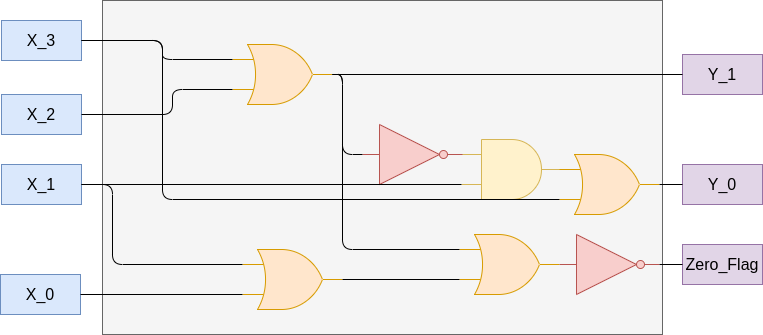
\includegraphics[width=.8\linewidth]{/home/noname/Documents/project_tiny/Ex3/20_doc/my-chapters/my-diagrams/Question2/spec.png}
	\caption{Sơ đồ logic của bộ LOPD 4bit.}
\end{figure}

Từ bộ LOPD 4-bit trên, ta triển khai bộ LOPD 8-bit và bộ LOPD 16-bit như sau:

\begin{figure}[H]
	\centering
	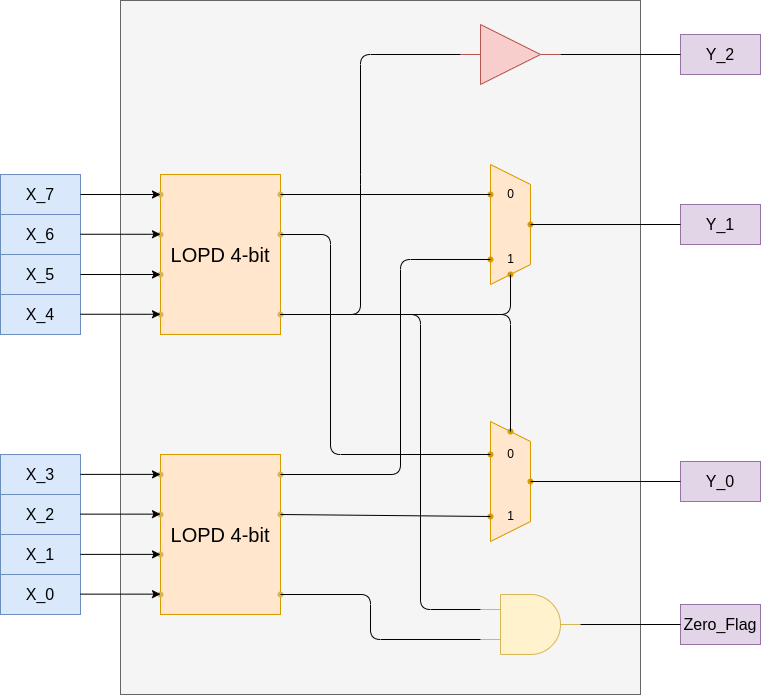
\includegraphics[width=.8\linewidth]{/home/noname/Documents/project_tiny/Ex3/20_doc/my-chapters/my-diagrams/Question2/LOPD_8bit.png}
	\caption{Sơ đồ logic của bộ LOPD 8bit.}
\end{figure}

\begin{figure}[H]
	\centering
	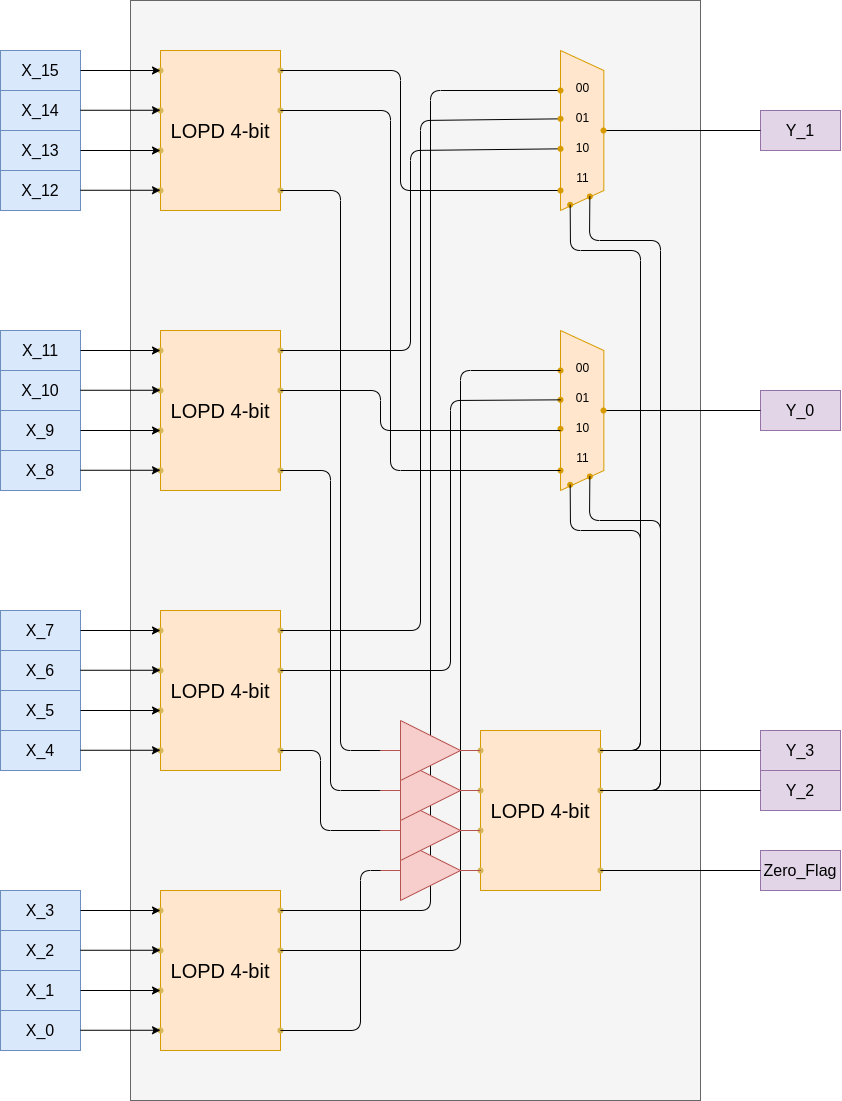
\includegraphics[width=.8\linewidth]{/home/noname/Documents/project_tiny/Ex3/20_doc/my-chapters/my-diagrams/Question2/LOPD_16bit.png}
	\caption{Sơ đồ logic của bộ LOPD 16bit.}
\end{figure}

Từ bộ LOPD 8-bit và LOPD 16-bit trên, ta ghép lại thành 24-bit với LOPD 8-bit vào vị trí 8-bit cao (từ $ 23 \rightarrow 16 $) và bộ LOPD 16-bit vào 16-bit thấp (từ $ 15 \rightarrow 0 $).

\begin{figure}[H]
	\centering
	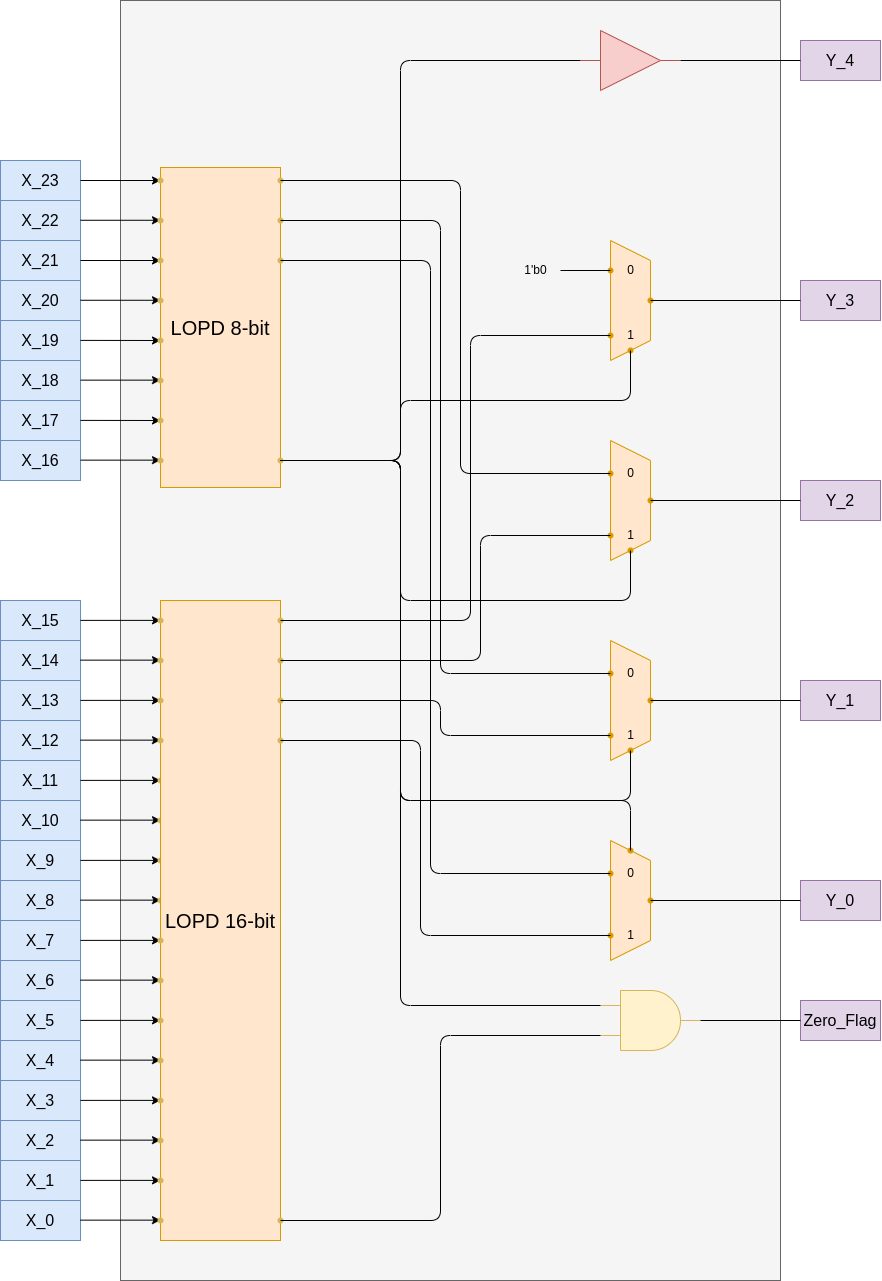
\includegraphics[width=.8\linewidth]{/home/noname/Documents/project_tiny/Ex3/20_doc/my-chapters/my-diagrams/Question2/LOPD_24bit.png}
	\caption{Sơ đồ logic của bộ LOPD 24-bit.}
\end{figure}

\answer{b}{Viết chương trình HDL mô tả mạch đã cho.}

\lstinputlisting[style=StyleCode, language=SystemVerilog, caption={Chương trình mô tả LOPD 4-bit.}]{/home/noname/Documents/project_tiny/Ex3/02_rtl/Question2/LOPD_4bit.sv}

\lstinputlisting[style=StyleCode, language=SystemVerilog, caption={Chương trình mô tả LOPD 8-bit.}]{/home/noname/Documents/project_tiny/Ex3/02_rtl/Question2/LOPD_8bit.sv}

\lstinputlisting[style=StyleCode, language=SystemVerilog, caption={Chương trình mô tả LOPD 16-bit.}]{/home/noname/Documents/project_tiny/Ex3/02_rtl/Question2/LOPD_16bit.sv}

\lstinputlisting[style=StyleCode, language=SystemVerilog, caption={Chương trình mô tả LOPD 24-bit.}]{/home/noname/Documents/project_tiny/Ex3/02_rtl/Question2/Question2.sv}

\answer{c}{Viết testbench cho mạch, thực hiện testbench với 100 mẫu và tính scoreboard của 100 mẫu đó.}

Đầu tiên nhóm em thưc hiện triển khai chứng minh kết quả đúng bằng giải thuật sau:

\begin{lstlisting}[style=StyleCode, language=SystemVerilog, caption={Giải thuật chứng minh kết quả của bộ LOPD 24-bit.}]
	function automatic logic [SIZE_LOP-1:0] Test_LOPD(
		input logic [SIZE_DATA-1:0]     f_i_data
	);
		logic [SIZE_DATA-1:0] t_temp;
		int cnt_position_1;
		begin
			t_temp = f_i_data;
			cnt_position_1 = 0;
			
			if(t_temp == 0) begin
				Test_LOPD = 0;
			end else begin
				while (t_temp[SIZE_DATA-1] == 0) begin
					t_temp = t_temp << 1;
					cnt_position_1 ++;
				end
				Test_LOPD = SIZE_DATA - cnt_position_1 - 1;
			end
		end
	endfunction
\end{lstlisting}

